



\chapter{Computational Aspects}
\label{sec:Computational Aspects}



\section{Sequential Version}
\label{sec:Sequential Version}




\section{Parallelization}
\label{sec:Parallelization}


The source code is implemented for an efficient parallelism with distributed memory, using the MPI~\cite{Forum2009}
standard for communication. The program uses the following MPI calls:
\begin{itemize}
	\item \lstinline{MPI_Init}, \lstinline{MPI_Finalize}, \lstinline{MPI_Comm_rank}, \lstinline{MPI_Comm_size} to set up basic MPI functionality
	\item \lstinline{MPI_Abort} to stop the program in case of an error
	\item \lstinline{MPI_Barrier}, \lstinline{MPI_Wtime} and \lstinline{MPI_Wtick} within the stopwatch class
	\item \lstinline{MPI_Bcast}, \lstinline{MPI_Reduce}, \lstinline{MPI_Allreduce} for simulation data exchange
\end{itemize}
Exclusively collective communication is used, an approach suitable for molecular simulations, where the cut-off radius is 
in the order of the simulation volume edge length. For MD simulations with $ms2$, only the force calculation is parallelized using the molecule decomposition according to Plimpton~\cite{plimpton1993}. The interaction matrix is rearranged such that the number of interaction partners is almost equally distributed in the matrix. This is achieved by calculating the interactions between molecule 1 and $N$ as interactions between molecules $N$ and 1, cf. Figure~\ref{ms2pic_plimpton}. The parallelization scheme then distributes the calculation among $N_P$ processors with an almost equal work load such that every processor executes $N/N_P$ rows of the interaction matrix. The master process reduces then all the force components to sum up the resulting molecular forces on each molecule.
\begin{figure}
	\begin{center}
		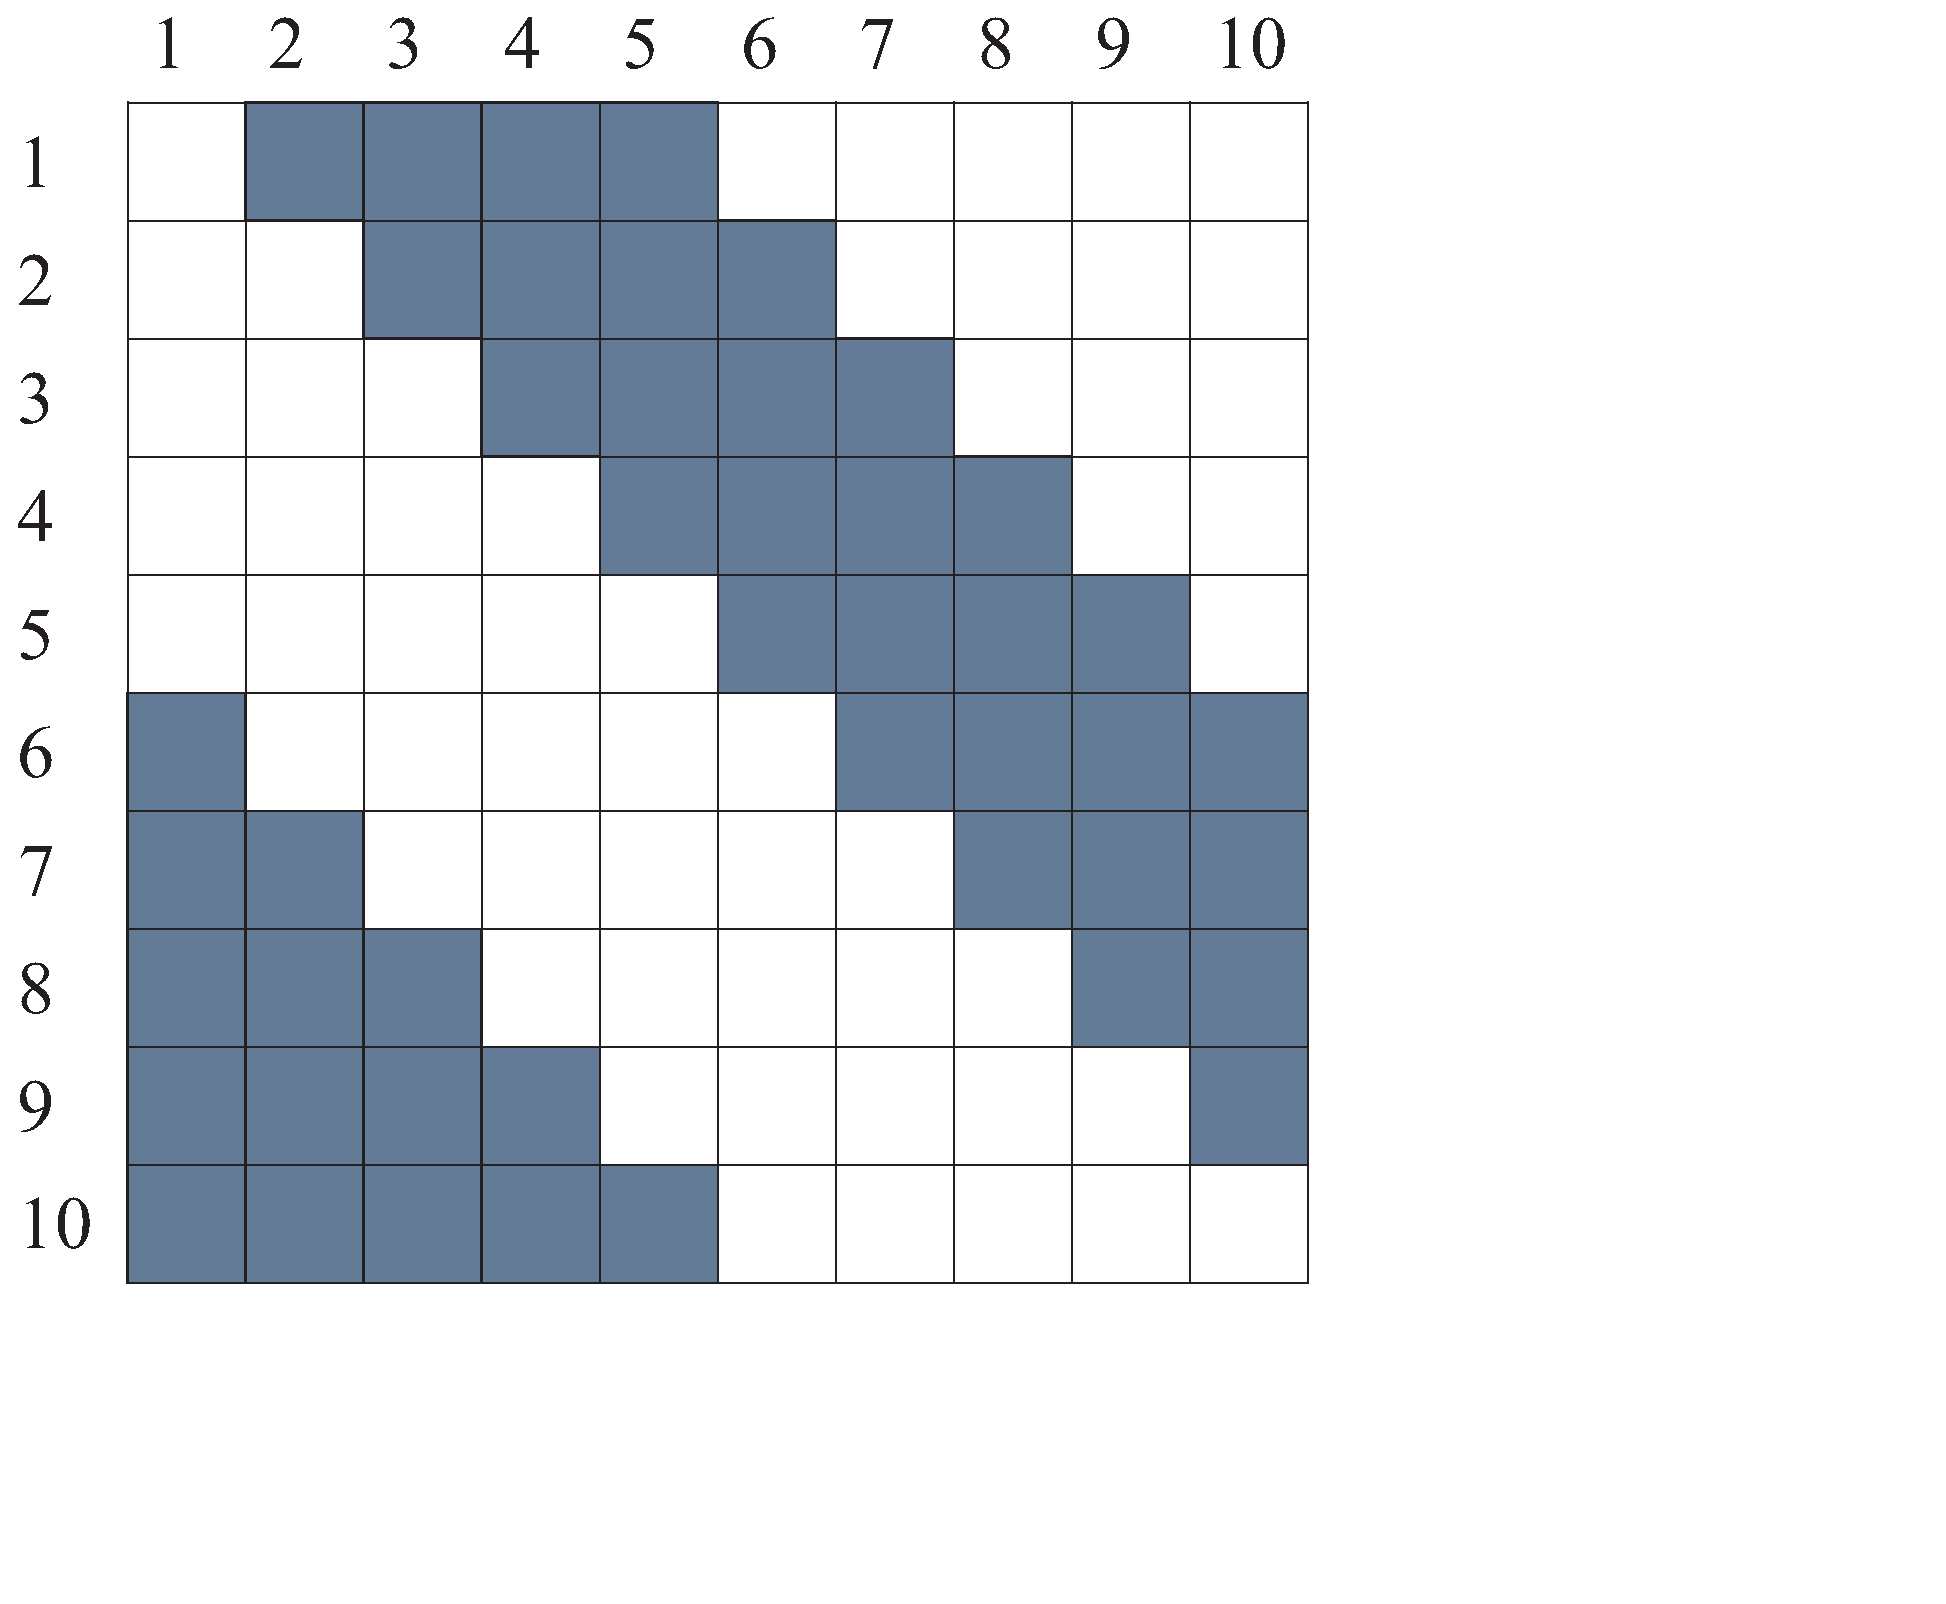
\includegraphics[width=7cm]{fig_Plimpton}
	\end{center}
	\caption{Schematic of the molecule decomposition parallelization by Plimpton~\cite{plimpton1993}.}
	\label{ms2pic_plimpton}
\end{figure}
\newline\noindent
% DE: Explanation of Triviral MC parallelization
The MC code is parallelized exploiting the stochastic nature of the simulation method. Starting from an equilibrated state in the simulation volume, the molecular configuration is copied multiple times into different volumes. Then, each copy runs  independently in parallel, but with a different random number seed, to calculate the thermodynamic properties. At the end, the data from all copies are gathered and averaged.



\section{Vectorization \& Memory}
\label{sec:Vectorization Memory}

The program $ms2$ specifically accounts for vector-parallel machines. All the main information needed in the computationally costly 
inner loops of the calculation, like the positions of the molecules and their sites, are stored in vectors that are accessed sequentially. 
This allows for an efficient use of memory on vector-parallel machines. \\ 
% 
For the evaluation of one configuration in $ms2$, e.g. the position vectors are loaded once and then distributed among all processors. 
Then, additional information like interaction partners of each individual molecule is computed, tabulated in vectors and communicated. 
The order of this data follows the order of all other vectors, e.g. the position vector. An example of a storage vector is shown 
in Table~\ref{vector_ex}.
The appropriate order allows for a serial access to the data in all vectors in the random access memory. 
Therefore, the calculations can be vectorized, increasing the efficiency. 
% 
\begin{table}[ht]
	\noindent
	\caption{Listing of the interaction partners for a molecule $i$, indicating the assembly in the storage vector.}
	\label{vector_ex}
	\begin{center}
		\begin{tabularx}{300pt}{c|X X X X X } 
			\hline
			\hline
			Molecule $i$ & \multicolumn{5}{c} {Interaction list for molecule $i$ within the storage vector}\\
			\hline
			1           &     2 & 4 & 6 & ... & 10 \\
			3           &       & 4 & 7 & ... & 10 \\
			4           &       &   & 8 & ... & 10 \\
			\hline
			\hline
		\end{tabularx}
	\end{center}
\end{table}


\section{Benchmarks/ Test case}
\label{sec:Benchmarks/ Test case}


% siehe erstes release paper Section 5


\section{Structure of program code}
\label{sec:Structure of program code}


This section discusses the code design and implementation issues of $ms2$ in detail. These explanations of the source code are 
intended to help understanding the program and to encourage the reader to further develop and improve the code.
\noindent 
New developers should get a smooth entry and the possibility to make fast adaptations to new problems.
Due to the experience of the core developers and the suitability for an efficient numerical code, Fortran90 was chosen as programming language. 
The program makes extensive use of the concepts introduced with Fortran90, notably modular programming.
% 
\noindent A wide variety of different simulation setups is possible, each requiring different 
computations. The most significant difference between the setups lies with the choice of MD or MC. While MD features extensive force 
calculations in order to update the molecular positions, MC is based on a Markov chain, where a molecular move is accepted with a certain 
probability. However, there are many other choices regarding the setup. This variety leads 
to a strong need for a highly modular structure, where modules have clear-cut interfaces. Given such a modularity, 
the appropriate functionalities can be combined to the desired simulation, while leaving out any unnecessary 
code\footnote{Unnecessary for the current setup.}. Besides avoiding if-statements at computationally demanding points and therefore 
leading to a better data flow, this allows for an efficient implementation of new functionalities, as existing modules can be used 
whenever feasible. In $ms2$, a stringent philosophy regarding modularization was followed, which is discussed in section~\ref{subsec_modstruc}.
% 
\noindent The runs need to be fast and scale well with increasing number of processors in order to achieve short response times. $ms2$ is parallelized with the Message Passing Interface~(MPI)~\cite{Forum2009}. While MD needs synchronization after 
every time step due to its deterministic nature, MC can be run embarrassingly parallel, only requiring synchronization at the very 
end of a run\footnote{Therefore, parallelization can be achieved by simply executing multiple MC runs simultaneously and averaging 
	over all runs, cf. section~\ref{subsec_parallel}.}. 
% 
\noindent Furthermore, the by far most expensive part of the code, calculating forces and potential energies, is highly vectorized 
and optimized.


-----

In order to keep the class hierarchy flat, $ms2$ does not make use of inheritance and hence polymorphism. 
E.g. the module \lstinline{ms2_site} contains the classes \lstinline{TSiteLJ126}, \lstinline{TSiteCharge}, \lstinline{TSiteDipole} 
and \lstinline{TSiteQuadrupole}, which have data and functionalities in common, but they are not derived from a common class.
\begin{figure}
	\begin{center}
		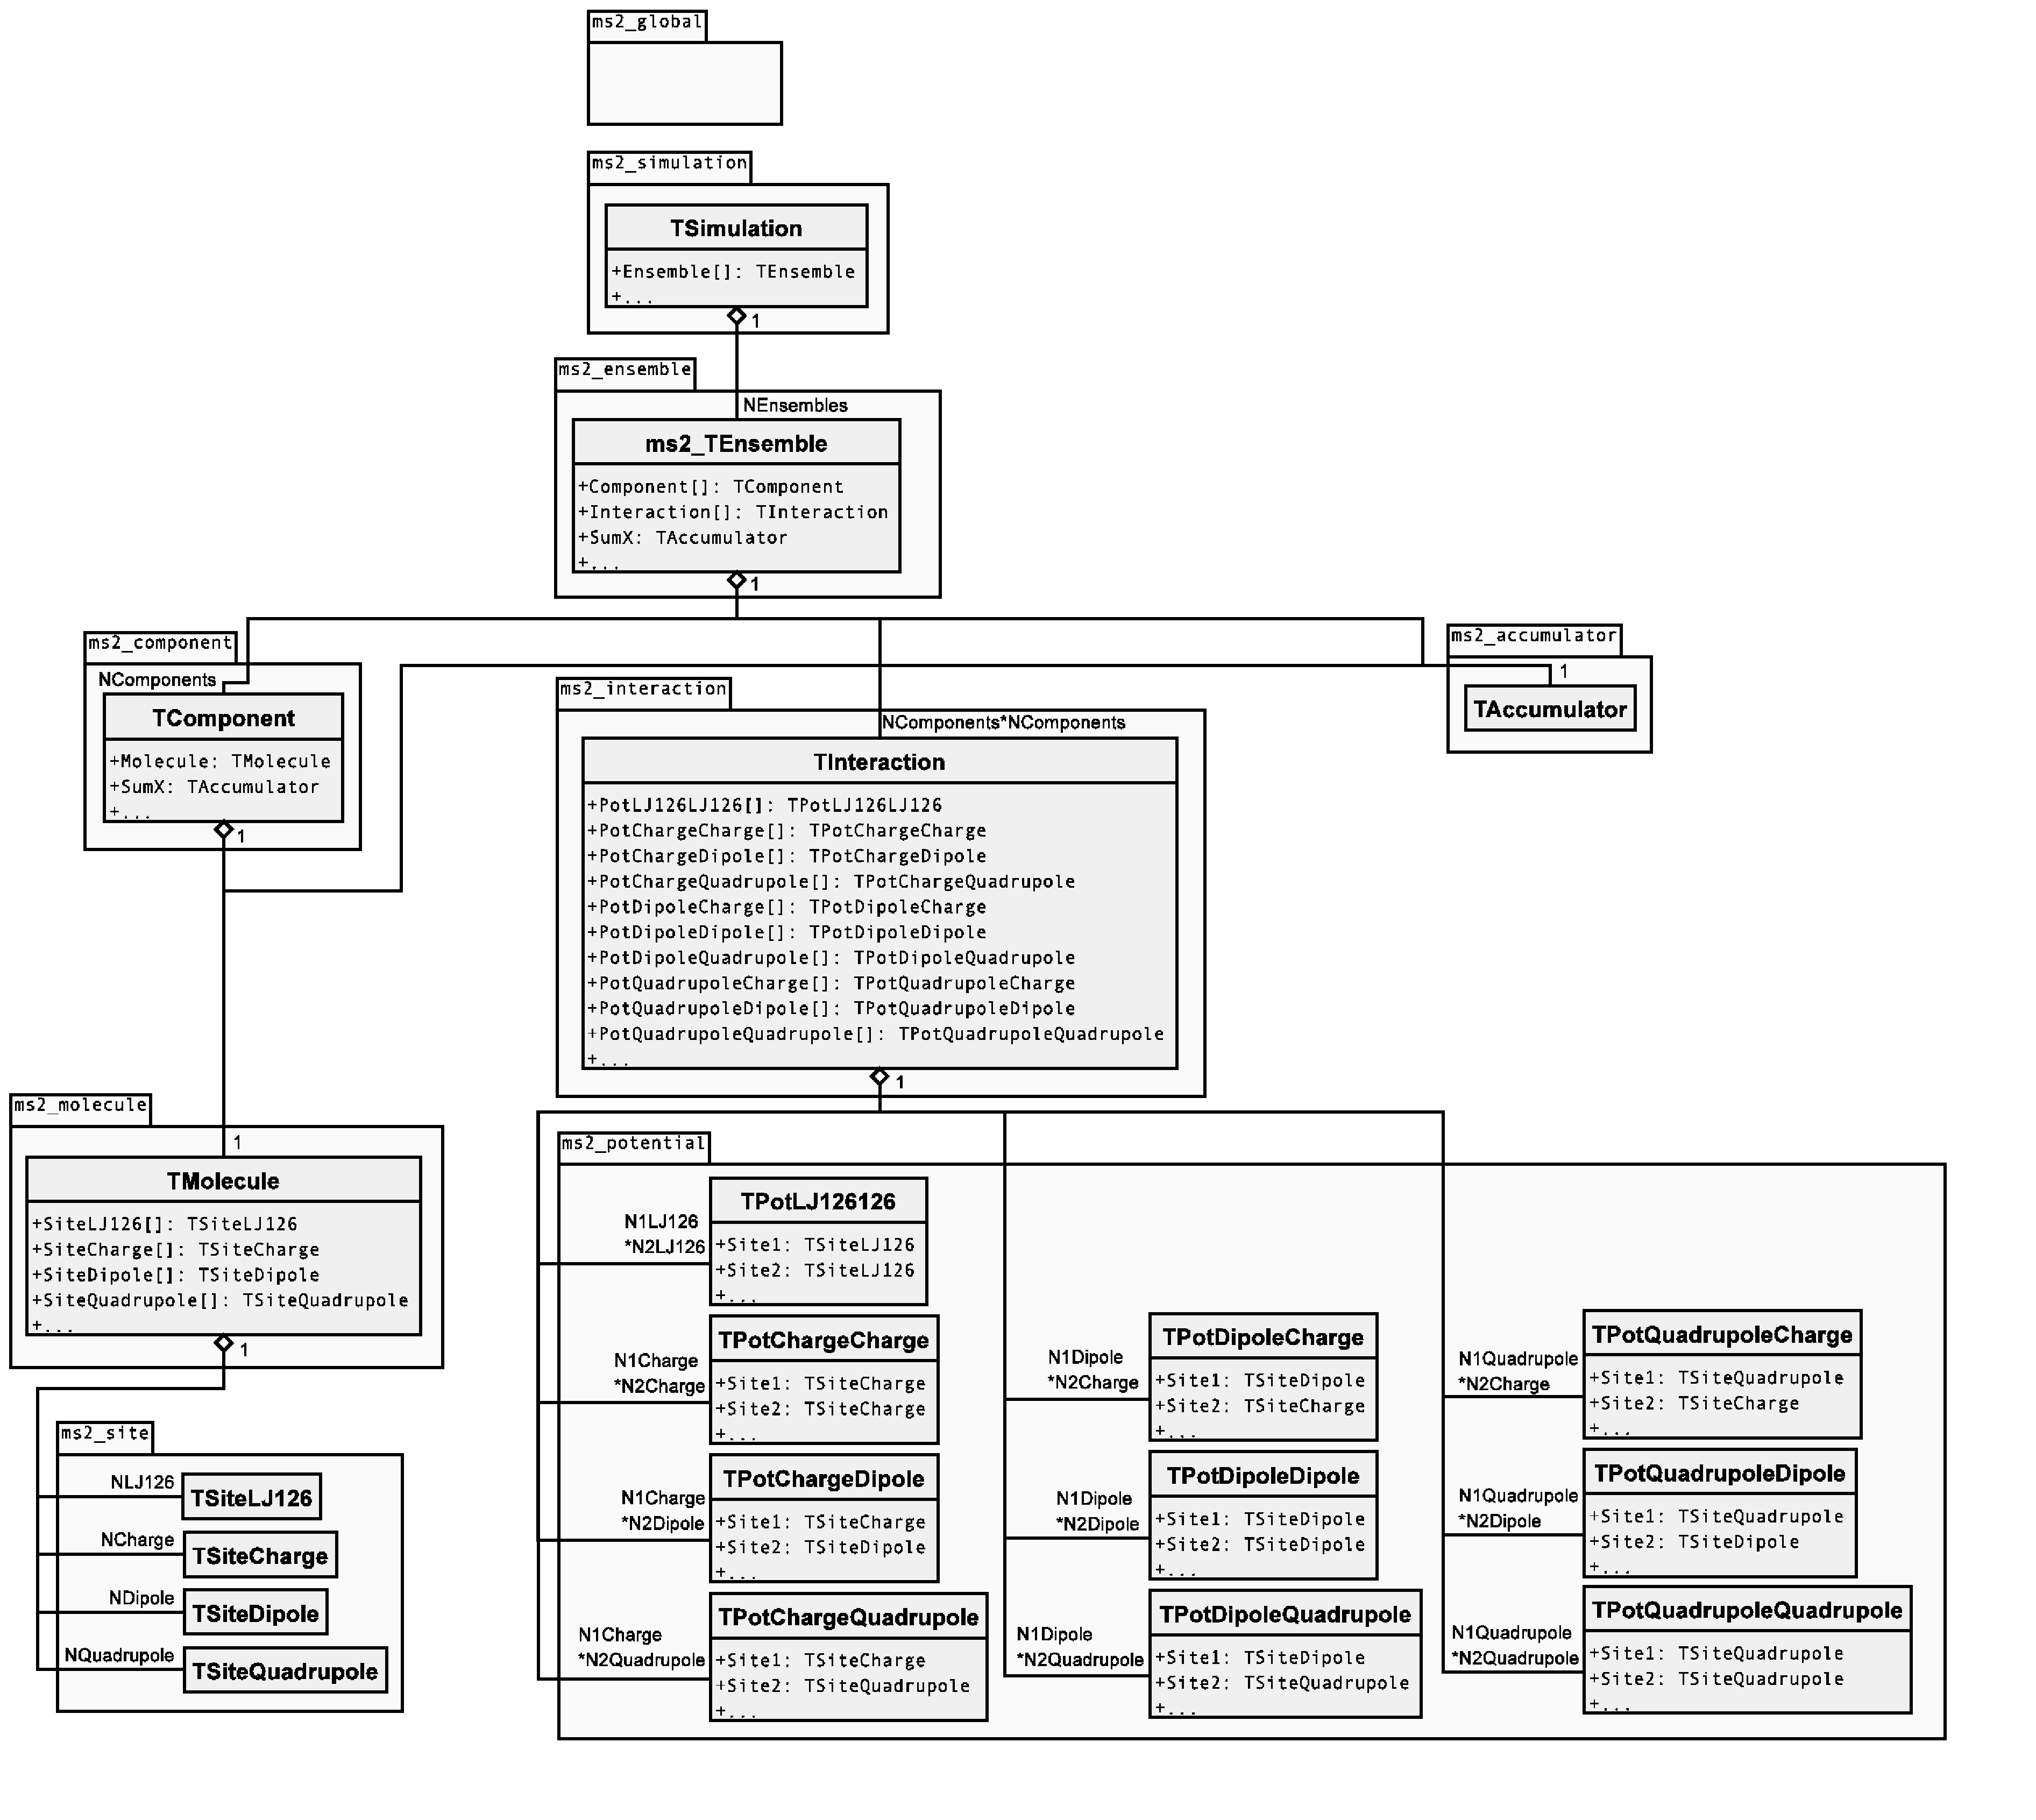
\includegraphics[width=\textwidth]{fig_ms2_modules_1.eps}
		\caption[aboveskip=0.5cm]{UML class diagram of $ms2$, showing object attributes.}
		\label{pic_ms2modules}
	\end{center}
\end{figure}
% 
\noindent The class structure and the relations between the classes is organized in six levels, as depicted in Figure~\ref{pic_ms2modules}.
% 
% 
% 
Every class is located on a certain level and hence has data and modules relevant to its level. 
The six levels are intuitive:
% 
\begin{enumerate}
	\item Global -- all data and functions of global use are handled. Scope: whole code
	\item Simulation -- setup and control of the simulation. Scope: simulation framework
	\item Ensemble -- the required ensemble is set up and initialized. Scope: molecular ensemble
	\item Component -- data and functions dealing with all molecules of a given molecule type. Scope: one molecule species
	\item Molecule -- data regarding the basic structure of a molecule. Scope: one molecule 
	\item Site -- position of sites with respect to a molecule. Scope: site of one molecule
\end{enumerate}


\textbf{First level - global}
The first level contains subroutines and variables that are needed globally in all parts of the simulation. The variables are mainly natural 
constants like the Boltzmann constant $k_{\mathrm B}$, the Avogadro constant $N_A$, etc. Additionally, variables defining the simulation 
setup for the given run are stored, e.g. the simulation technique and the ensemble type. 
These variables determine the type of calculation and are assigned according to user specifications on subsequent levels in $ms2$.
Subroutines that are stored on this level are also of global use in $ms2$. These are basic routines for input into the simulation tool and 
output into files, as well as more advanced routines for automated communication between hardware and program via signals. The latter routines 
are of particular interest for running $ms2$ on high performance clusters, where possible data loss can be avoided by automated communication 
between cluster nodes and the program.
% 
\textbf{Second level - simulation}
On the second level, the simulation flow is controlled. The simulation is initiated, started and sustained. This includes controlling the 
length of the simulation and its output, which is further discussed in section~\ref{sec_io}. User specifications concerning the simulation 
setup are read and the corresponding  global variables are assigned accordingly. Furthermore, all simulation quantities and averages are 
analyzed and written to file.
% 
\textbf{Third level - ensemble}
On the third level, the simulation is organized according to the desired ensemble specified by the user.
The respective ensemble is initialized, by characterizing the ensemble setup and defining e.g. the volume and the composition of the 
molecular species in the simulation volume. 
\noindent In addition, the initial positions and velocities of all molecules are distributed. Furthermore, the routines for the subsequent 
simulation are assigned on this level. The time evolution or the Markov chain, respectively, is performed and the ensemble averages 
of thermodynamic properties are calculated during the simulation run. 
% 
\textbf{Fourth level - component}
On this level, the molecule species (component) and their interactions are addressed. The class structure has three distinct 
branches. While the first branch deals with issues regarding structure and properties of one component at a time, 
the second branch deals with interactions between molecules of one or two components. 
The third branch contains all routines for the accumulation of data, determining the average value of the data as well as their statistical 
uncertainties. The first two branches will be discussed in more detail.\\
The first branch deals with the structure of one individual component. An instance of the class component stores center of mass 
position, orientation, velocity etc. of every molecule of one species, e.g. H$_2$O. The contained modules deal with calculations 
all molecules of this species, e.g. modules for solving Newton's equations of motion, kinetic energy calculation, atom to molecule 
transformation and vice versa. Furthermore, this branch is responsible for the correct initialization. 
It reads the molecular model for every component, calculates positions, introduces the reduced quantities, etc.\\
The second branch deals with interactions between molecules of one or two components. Therefore, this branch contains all force and 
potential energy calculations, which are the computationally most expensive parts by far. This branch is highly vectorized to achieve a fast 
calculation, in particular if executed in vector-parallel. The modules in this branch are simulation technique specific, i.e. MD or MC. 
\noindent
In a MD simulation, first, the interaction partners of every molecule are determined,  i.e. other molecules or sites within the 
cut-off radius. Then the interaction energies and virial contributions as well as the resulting forces and torques are calculated and 
summed up for every molecule. \\  
In a MC simulation, the modules are designed to calculate only the energy and the virial. Forces are not calculated and the 
corresponding algorithms are therefore entirely omitted in these modules.
\noindent
For MD, all interactions of one component-component pair\footnote{Please note that a component-component pair can consist of 
	one component paired with itself.} are calculated in one call of the module and they are therefore called once for every component-component 
pairing. For MC, the modules are finer-grained, calculating all interactions of one component-component pair by determining every 
molecule-molecule interaction individually. The corresponding modules are thus called more frequently than in case of MD.
% 
\textbf{Fifth level - molecule}
The basic information on molecules is stored on this level, such as mass, moment of inertia tensor, 
rotational degrees of freedom, etc. Higher level modules access this data via the class molecule.

\textbf{Sixth level - site}
Here, the assembly of a molecule is stored. The data is used by higher level modules to calculate the site positions 
from the molecular positions and orientations. This allows for the calculation of site-site interactions. It should be noted that $ms2$ only 
integrates (MD) or accepts (MC) center of mass positions and orientations. Site specific data is calculated for every simulation step on the fly.
% 

\textbf{Example}
The modular structure is discussed by highlighting the calculation process of a MD simulation of a pure fluid modeled by two LJ~sites 
and two point charges in the $NVT$ ensemble. 
During the initialization process, the modules for memory allocation and definition of the simulation scenario are executed. 
This process is not unique for one of the hierarchical levels, but takes places on all levels, cf. Figure~\ref{pic_ms2modules}. 
On level one, the simulation is delimited to "molecular dynamics", therefore all modules concerning MC simulation are neglected entirely. 
On level two, the "initialization" modules define the simulation environment by setting ensemble specific properties like simulation volume, 
temperature as well as the thermostat and integration scheme, etc. While the use of the first modules mentioned here is required 
in each simulation, independently of MD or MC, e.g. the trajectory calculation is specific for MD. However, the modular 
structure helps keeping the efficiency of the program by initiating only the simulation-specific molecule propagation.
The same effect of modules can be found in the initiation process on lower levels. Here, the exact composition of the molecular species 
in the simulation volume (module component), the description of the molecule (module molecule) and the storage of the positions, 
velocities and forces of all LJ~sites and charges (module sites) is determined. 
All other modules, like treating additional components for mixtures or containing characteristic properties of dipoles or 
quadrupoles, are fully omitted by $ms2$, since these are not used throughout this simulation.
% 
% 
Once the simulation has been initialized, a set of modules is invoked, which deals with maintaining the molecular simulation. 
On level one, this includes modules of global use for any simulation, e.g.~limiting the execution time, etc. 
On level two, Newton's equations of motion are numerically integrated, requiring information about the fluid's composition, 
the positions and orientations of the molecules etc. provided by modules of the respective level. The thermostat is applied and the 
calculation of thermodynamic properties is performed. The forces, torques and energies are calculated  in the second branch 
on the level component. For a MD simulation, this covers routines for the calculation of energies as well as forces at the same time, 
whereas in contrast for a MC simulation, the modules only calculate energies and virial contributions. 
% 
A further set of modules deals with the accumulation of data. These modules are designed to store data and evaluate the statistics of 
the produced data. The actual thermodynamic properties are calculated on the ensemble level. 
% 
The last set of modules deals with the output, where the results of the molecular simulation are written to file. These modules are called 
independent on the user settings in all simulation scenarios. 

